\chapter{GRAPHS}


\section{Introduction}
A \eax{graph} is a pair $G = (V,E)$, where $V$ is a set whose elements are called \eax{vertices} and $E \subseteq V \times V$ is a set of unordered pairs $\{v_{1},v_{2}\}$ of vertices, whose elements are called edges. Here, $(v_{1},v_{2})$ and $(v_{2},v_{1})$ are undistinguishable, and are simply denoted by $\{v_{1},v_{2}\}$ or $v_{1}v_{2}$.
\begin{figure}[h]
    \centering
    \begin{tikzpicture}[scale=1,
        every node/.style={circle, draw=\subjectcolor!80!black, fill=\subjectcolor!40!white, inner sep=2pt}]
        % Vertices
        \node (A) at (0, 0.2) {A};
        \node (B) at (2.1, -0.1) {B};
        \node (C) at (1.2, 1.6) {C};
        \node (D) at (3.1, 1.4) {D};
        \node (E) at (4.2, 0.1) {E};

        % Edges
        \draw (A) -- (B);
        \draw (B) -- (C);
        \draw (C) -- (A);
        \draw (B) -- (D);
        \draw (D) -- (E);
    \end{tikzpicture}
\end{figure}

The above shows a simple undirected graph on five vertices $V=\{A,B,C,D,E\}$ with edges $E=\{AB,AC,BC,BD,DE\}$. Here, simple and undirected are also terms to be defined in the context of graph theory.

\begin{definition}
    A graph is called a \eax{simple graph} if it has no loops (edges connecting a vertex to itself) and no multiple edges (more than one edge connecting the same pair of vertices). Otherwise, it is termed a \eax{multigraph}. A graph is called an \eax{undirected graph} if its edges have no orientation; that is, the edge $uv$ is identical to the edge $vu$. Otherwise, it is termed a \eax{directed graph}.
\end{definition}

In directed graphs, or \eax{digraph}s, one deals with $G = (V,E,s,t)$, where $s:E \to V$ gives the \eax{source node} of an edge and $t:E \to V$ gives the \eax{target node} of an edge. In this edge set $E$, $uv \neq vu$, unlike the case of a simple graph.

Structure-preserving maps are useful in graph theory too.

\begin{definition}
    Suppose we have two graphs $G = (V(G),E(G))$ and $H = (V(H),E(H))$. A function $f:V(G) \to V(H)$ is said to be a \eax{graph homomorphism} if $f$ preserves adjacency; that is, if $v_{1}v_{2} \in E(G)$, then $f(v_{1})f(v_{2}) \in E(H)$. If $f$ is also bijective and $f$ and $f^{-1}$ are both graph homomorphisms, then $f$ is termed a \eax{graph isomorphism}.
\end{definition}

We also term the group $\Aut(G)$ as the group of all graph isomorphisms of $G$, with the group operation of composition.

\begin{definition}
    Suppose we have two digraphs $G_{1} = (V_{1},E_{1},s_{1},t_{1})$ and $G_{2} = (V_{2},E_{2},s_{2},t_{2})$. A \eax{digraph homomorphism} is two maps $f_{V}:V_{1} \to V_{2}$ and $f_{E}:E_{1} \to E_{2}$ such that
    \begin{align}
        s_{2}(f_{E}(e)) = f_{V}(s_{1}(e)) \quad \text{ and } \quad t_{2}(f_{E}(e)) = f_{V}(t_{1}(e)).
    \end{align}
    That is, the source node of every image edge is the image node of every source node, and the target node of every image edge is the image node of every target node.
\end{definition}

One also discusses the neighbours of nodes.

\begin{definition}
    The \eax{degree of a node}, or the \eax{valency of a node}, is simply defined as the number of edges incident with the vertex. If $v$ is such a node in a graph $(V,E)$, then $\deg(v) = \#\{u \in V \mid vu \in E\}$. In digraphs, one defines the \eax{out-degree of a node} $v$ as the number of edges with $v$ as the source node, and the \eax{in-degree of a node} $v$ as the number of edges with $v$ as the target node.
\end{definition}

A \eax{regular graph} is one where every vertex has the same degree. We now discuss the first ever theorem (historically) in graph theory.

\begin{theorem}
    A finite (simple) graph $G$ has an even number of vertices of odd degree.
\end{theorem}

\begin{proof}
    Let $G = (V,E)$ be a graph. One can deduce that
    \begin{align}
        2 \cdot \# E(G) = \sum_{v \in V(G)} \deg(v).
    \end{align}
    Thus, there must be an even number of vertices of odd degree to keep the term on the left even.
\end{proof}


\section{Walks, Paths, and Cycles}

\begin{definition}
    A \eax{walk on a graph} $G$ is an alternating sequence of vertices and edges 
    \begin{align}
        (v_{0},e_{1},v_{1},e_{2},v_{2},\ldots,e_{k},v_{k})
    \end{align}
    such that for all $i$, $e_{i}$ is an edge between $v_{i-1}$ and $v_{i}$. The \eax{length of a walk}, in this case, is termed $k$.
\end{definition}


\begin{definition}
    If the edges $e_{1},e_{2},\ldots,e_{k}$ are distinct, then the walk is called a \eax{path on a graph}. A \eax{simple path} is one where the vertices $v_{0},v_{1},\ldots,v_{k}$ are also all distinct. Finally, a \eax{simple closed path}, or a \eax{cycle on a graph}, is one where $v_{0} = v_{k}$ and the rest are distinct.
\end{definition}

A \eax{metric on a graph} between two vertices $d(v_{1},v_{2})$ is defined as the length of the shortest walk between $v_{1}$ and $v_{2}$. This walk is always a path since if it's not, there is a repetition of edges, and appropriate middle edges and vertices can be deleted to form a path or a shorter walk. If no such path exists, then $d(v_{1},v_{2}) = \infty$. Thus, a finite \eax{connected graph} $G$ is one where $d(v_{1},v_{2}) < \infty$ for all $v_{1},v_{2} \in V(G)$.\\ \\
\textit{August 21st.}

\subsection{The K\"onigsberg Bridge Problem}

The following figure illustrates the famous problem of the \eax{K\"onigsberg bridge problem}.

\begin{figure}[h]
    \centering
    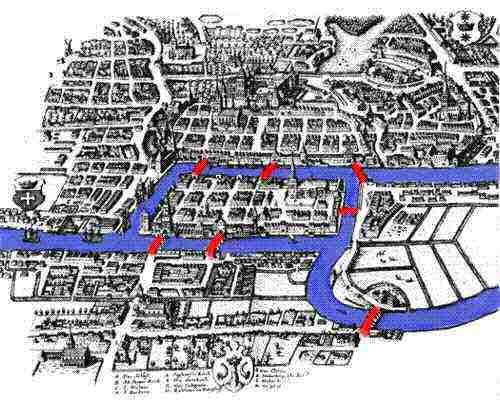
\includegraphics[width=0.3\textwidth]{chapters/konigsberg.jpg}
    \caption{The Seven Bridges of K\"onigsberg}
    \label{fig:konigsberg}
\end{figure}

Euler asked the question if one could cross each of the seven bridges exactly once and come back to the same side of the riverbank; this is formally considered as the first ever problem in graph theory.

Here, an \eax{Eulerian circuit} is defined, which is a closed path using every edge in the graph exactly once. A graph with an Eulerian circuit is termed an \eax{Eulerian graph}.

\begin{figure}[h]
    \centering
    \begin{tikzpicture}[scale=1.2,
        every node/.style={circle, draw=\subjectcolor!80!black, fill=\subjectcolor!40!white, inner sep=2pt}]
        
        % Nodes
        \node (A) at (0, 1.5) {A}; % North bank
        \node (B) at (0, 0) {B};   % South bank
        \node (C) at (2, 0.75) {C}; % Island (Kneiphof)
        \node (D) at (4, 0.75) {D}; % East bank or another land mass

        % Edges (bridges)
        \draw (A) -- (B);         % Bridge 1
        \draw (A) -- (C);         % Bridge 2
        \draw (A) -- (C);         % Bridge 3 (double line)
        \draw (B) -- (C);         % Bridge 4
        \draw (B) -- (C);         % Bridge 5 (double line)
        \draw (A) -- (D);         % Bridge 6
        \draw (C) -- (D);         % Bridge 7

    \end{tikzpicture}
    \caption{Graph Representation of the Seven Bridges of K\"onigsberg}
    \label{fig:konigsberg_graph}
\end{figure}
(Above graph to be fixed.)

\begin{theorem}
    A finite multigraph $G$ is Eulerian if and only if $G$ is connected and is a edge-disjoint union of cycle $G = C_{1} \cup C_{2} \cup \cdots \cup C_{m}$ where $C_{i}$'s are cycles with no common edges.
\end{theorem}

\begin{proof}
    Suppose $G = C_{1} \cup C_{2} \cup \cdots \cup C_{m}$ where $C_{i}$'s are edge-disjoint cycles. For $m = 2$, choose $v \in V(C_{1}) \cap V(C_{2})$; such a $v$ must exist or else the graph is disconnected. Starting at $v$, exhaust all edges in $C_{1}$ using the trivial Eulerian circuit and return to $v$. Do the same with $C_{2}$, and you have found the Eulerian circuit. Now apply the induction hypothesis; for an arbitrary $m$, choose $v \in V(C_{1} \cup C_{2} \cup \cdots \cup C_{m-1}) \cap V(C_{m})$. Again, such a $v$ must exist since $G$ is connected. Starting at $v$, exhaust all edges in $C_{1}$ using the trivial Eulerian circuit and return to $v$, then use the Eulerian circuit in $C_{1} \cup C_{2} \cup \cdots \cup C_{m-1}$ formed via the induction hypothesis.

    For the converse, an Eulerian circuit on the graph involves all edges and returns to the same vertex, so $G$ must be connected. To show the disjoint union of cycles, find a cycle in the Eulerian circuit; there must exist at least one since, if not, the circuit itself is a cycle. Delete the edges from this cycle, and join the starting vertex and ending vertex in of this cycle in the circuit. Repeat the same until the resulting Eulerian circuit is a cycle. The disjoint union of this cycle and the cycles removed is the starting circuit.
\end{proof}

One can show a better result.

\begin{theorem}
    A finite multigraph $G$ is Eulerian if and only if $G$ is connected and every vertex has an even degree.
\end{theorem}

\begin{proof}
    If $G$ is Eulerian, then $G$ is connected by the previous theorem, and $G = C_{1} \cup C_{2} \cup \cdots \cup C_{m}$, a union of disjoint cycles. Also, for $v \in V(G)$,
    \begin{align}
        \deg_{G}(v) = \sum_{i=1}^{m} \deg_{C_{i}}(v) = 2 \left( \sum_{i=1}^{m} \1_{\{v \in C_{i}\}} \right).
    \end{align}
    Thus, $\deg_{G}(v)$ is even for all $v \in V(G)$.

    For the converse implication, assume $G$ is connected and every vertex has an even degree. We will show that $G$ is Eulerian. Start by choosing any cycle $C_{1}$ in $G$. Remove the edges of $C_{1}$ from $G$ to form a subgraph $G'$. Since every vertex in $G$ has even degree, removing the edges of $C_{1}$ leaves every vertex in $G'$ with even degree. If $G'$ is connected, repeat the process to find another cycle $C_{2}$ in $G'$. Continue this process until no edges remain. If $G'$ is disconnected at any step, then each connected component of $G'$ must also have all vertices of even degree. By the same argument, we can find cycles in each connected component and remove their edges. Eventually, all edges of $G$ are partitioned into disjoint cycles. Since $G$ is connected, these cycles can be combined into a single Eulerian circuit by appropriately traversing edges between cycles. Thus, $G$ is Eulerian.
\end{proof}

\section{Adjacency}

For a simple graph $G = (V,E)$, an \eax{adjacency matrix} can be defined of dimension $\# V \times \# V$, with $a_{v,w} = 1$ if $vw \in E$, and $a_{v,w} = 0$ otherwise. For a multigraph, $a_{v,w}$ is the number of edges between vertices $v$ and $w$. Similarly, for a directed graph, $a_{v,w} = 1$ if $vw \in E$ and $a_{w,v} = 0$ otherwise. For an undirected graph, the adjacency matrix $A$ is symmetric and consists of only 1's and 0's. 

\begin{figure}[h]
    \centering
    \begin{tikzpicture}[scale=1.2,
        every node/.style={circle, draw=\subjectcolor!80!black, fill=\subjectcolor!40!white, inner sep=2pt}]
        
        % Nodes with slight deviations
        \node (A) at (0.1, 1.6) {$v_{1}$};
        \node (B) at (1.6, 1.4) {$v_{2}$};
        \node (C) at (-0.1, -0.1) {$v_{3}$};
        \node (D) at (1.4, 0.1) {$v_{4}$};

        % Edges
        \draw (A) -- (B);
        \draw (A) -- (C);
        \draw (B) -- (D);
        \draw (C) -- (D);
        \draw (B) -- (C);

    \end{tikzpicture}
    \caption{A simple graph with four vertices}
    \label{fig:graph_example}
\end{figure}
The adjacency matrix for the graph in Figure~\ref{fig:graph_example} is given as
$
A =
\begin{bmatrix}
0 & 1 & 1 & 0 \\
1 & 0 & 1 & 1 \\
1 & 1 & 0 & 1 \\
0 & 1 & 1 & 0
\end{bmatrix}
$. For two graphs $G_{1}$ and $G_{2}$ to be isomorphic, one can show that $A(G_{1})$ must be similar to $A(G_{2})$. Moreover, to count the number of walks from $v$ to $w$ of length $k$, one can use the $k$-th power of the adjacency matrix: the entry $(i,j)$ of $A^{k}$ gives the number of walks of length $k$ from vertex $v_{i}$ to vertex $v_{j}$.

\textit{August 28th.}
\begin{theorem}
    Let $G = (V,E)$ be a simple graph with $n$ vertices $V = \{1,2,\ldots,n\}$ and adjacency matrix $A$. Then the $(i,j)^{\text{th}}$ entry of $A^{k}$ gives the number of walks of length $k$ from vertex $i$ to vertex $j$.
\end{theorem}

\begin{proof}
    $k = 1$ is trivial, as a walk of length $1$ is just showing there exists an edge between the two vertices. Let $k = 2$. Then the $(i,j)^{\text{th}}$ entry of $A^{2}$ is given as
    \begin{align}
        (A^{2})_{i,j} = \sum_{m=1}^{n} a_{im} a_{mj}
    \end{align}
    where $a_{ij}$ is 1 if $i$ and $j$ are neighbours and zero otherwise. Thus, $a_{im}a_{mj}$ represents if vertex $m$ is an immediate intermediate vertex between $i$ and $j$. Thus, the number of walks of length 2 from $i$ to $j$ is equal to the number of such intermediate vertices $m$.

    Assume the result holds for an arbitrary $k$; that is, $(A^{k})_{i,j}$ gives the number of walks from $i$ and $j$ of length $k$. Then, for $k+1$, we have
    \begin{align}
        (A^{k+1})_{i,j} = \sum_{m=1}^{n} (A^{k})_{i,m} a_{mj}.
    \end{align}
    Any walk from $i$ to $j$ must have a neighbour of $j$ at the $k^{\text{th}}$ step. By the induction hypothesis, $(A^{k})_{i,m}$ represents the number of walks from $i$ to $m$ of length $k$. Thus, the total number of walks from $i$ to $j$ of length $k+1$ is the sum over all possible intermediate vertices $m$.
\end{proof}

\begin{theorem}
    Let $\lambda_{1},\ldots,\lambda_{n}$ be the eigenvalues of $A(G)$ where $G = (V,E)$ is a simple graph. Then the number of closed walks of length $k$ is given by $\sum_{i=1}^{n} \lambda_{i}^{k}$.
\end{theorem}
\begin{proof}
    The number of such closed walks of length $k$ is, clearly, $\tr A^{k}$. The eigenvalues of $A^{k}$ are $\lambda_{1}^{k},\ldots,\lambda_{n}^{k}$, and the trace is the sum of all eigenvalues; the result immediately follows.
\end{proof}

\begin{remark}
    \begin{itemize}
        \item For $k = 2$, $\frac{1}{2}\tr A^{2}$ provides the number of edges in the graph.
        \item For $k = 3$, $\frac{1}{6}\tr A^{3}$ provides the number of triangles in the graph.
    \end{itemize}
\end{remark}

\begin{example}
    $G$ is connected if and only if the largest eigenvalue of $A$ has multiplicity 1. This is known as the \eax{Perron-Frobenius theorem} will be taken as granted for now, without providing a proof.
\end{example}

\begin{proposition}
    For any eigenvalue $\lambda$ of $G = (V,E)$, it holds that $\abs{\lambda} \leq \max_{v \in G} \deg(v)$.
\end{proposition}
\begin{proof}
    Pick a corresponding eigenvector $x \neq 0$ with $Ax = \lambda x$, where $A$ is the adjacency matrix. Pick $x_{j} = \norm{x}_{\infty} = \max_{i} \abs{x_{i}}$. Then we have
    \begin{align}
        \abs{\lambda}\abs{x_{j}} = \abs{\lambda x_{j}} = \abs{\sum_{i=1}^{n} A_{ji} x_{i}} \leq \sum_{i=1}^{n} A_{ji} \abs{x_{i}} \leq \abs{x_{j}} \sum_{i=1}^{n} A_{ji} = \abs{x_{j}} \deg (j) \implies \abs{\lambda} \leq \deg (j) \leq \max_{v \in G} \deg(v).
    \end{align}
\end{proof}

\begin{proposition}
    Let spectrum of $G = \{\lambda_{1},\ldots,\lambda_{n}\}$ be the list of eigenvalues where $\lambda_{1} \leq \lambda_{2} \leq \cdots \leq \lambda_{n}$. Then
    \begin{align}
        \frac{1}{n}\sum_{v \in G} \deg(v) \leq \lambda_{n} \leq \max_{v \in G} \deg(v).
    \end{align}
\end{proposition}

\begin{proof}
    Let $e = (1\;1\;\cdots\;1)^{t}$, and let $d = Ae = (\deg(v_{1})\;\deg(v_{2})\;\cdots\;\deg(v_{n}))^{t}$. Then $e^{t}Ae = ed = \sum_{v \in G} \deg(v)$. Then $\sup_{\norm{x}=1}\ip{x,Ax} = \lambda_{\max}(A) \geq \frac{e^{t}}{\sqrt{n}} A \frac{e}{\sqrt{n}} = \frac{1}{n}\sum_{v \in G} \deg(v)$. The second inequality is just the one above.
\end{proof}

\begin{theorem}
    A finite multigraph $G$ is Eulerian if and only if $G$ is connected and every vertex has an even degree.
\end{theorem}
\begin{proof}
    If $G$ is Eulerian, then it is connected and every vertex has an even degree by definition. Conversely, suppose $G$ is connected and every vertex has an even degree. Take `a' longest trail, one where edges are not repeated, starting at $x \in V(G)$. We claim that this trail is actually closed. Let, if possible, the endpoint be $y \neq x$. There must have been an ``entering'' edge followed by an ``exiting'' edge. In the last step, one has entered $y$ but never exited it. So, an odd number of edges incident with $y$ appear in this trail. As $\deg(y)$ is even, there must be an unused edge incident with $y$. If we append that edge to the trail, we have a longer trail, contradicting our assumption.

    We make another claim that this trail exhausts all edges. To show this, start by deleting all edges appearing in this trail. Assume that the graph so-obtained has at least one edge. In the trail, $T$, if a vertex $y$ appears all its incident edges must also appear. Let $z$ be a vertex not appearing on $T$. Then none of the vertices in $T$ are neighbours of $z$, showing $G$ not connected which is a contradiction.
\end{proof}


\subsubsection{Hamiltonian Graphs}
\textit{August 29th.}

\begin{definition}
    A cycle in $G = (V,E)$ is said to be a \eax{Hamiltonian cycle} if the vertices in the cycle are all distinct, except the starting and ending vertices, and all vertices are exhausted. A simple graph with a Hamiltonian cycle is termed a \eax{Hamiltonian graph}.
\end{definition}

\begin{example}
    \begin{itemize}
        \item Trivially, all polygons with $n$ vertices $C_{n}$ are Hamiltonian graphs.
        \item The complete graph $K_{n}$ is Hamiltonian for all $n \geq 3$.
    \end{itemize}
\end{example}

If $G = (V,E)$ is a graph, then a \eax{subgraph} $H = (V(H),E(H))$ is such that $V(H) \subseteq V(G)$ and $E(H) \subseteq V(H)$ where $E(H)$ are edges connecting vertices in $V(H)$. A \eax{spanning subgraph} is such that $V(H) = V(G)$. We note that $G$ is Hamiltonian if and only if $C_{n}$ is a spanning subgraph of $G$.

Our goal now is to find a characterizing condition for Hamiltonian graphs (similar to the characterization of Eulerian graphs), and if a graph is Hamiltonian, then finding the (a) Hamiltonian cycle. The proof of providing a characterization is out of the scope of this course, while the latter problem is NP-hard and not always computationally tactible.


\begin{definition}
    The \eax{Hamiltonian closure of a graph} $G$, denoted by $\cl(G)$, is the graph obtained by repeatedly adding an edge between non-adjacent vertices $u,v$ such that $\deg(u)+\deg(v) \geq n = \#V(G)$.
\end{definition}

\begin{proposition}
    With $\#V(G) = n \geq 3$, let $G$ be a simple graph. If $\deg(v) \geq \frac{n}{2}$ for all $v \in V(G)$, then $G$ is Hamiltonian.
\end{proposition}

\begin{lemma}
    A graph $G$ is Hamiltonian if and only if $\cl(G)$ is Hamiltonian.
\end{lemma}
\begin{proof}
    If $G$ is Hamiltonian, then clearly $\cl(G)$ is Hamiltonian since adding edges cannot remove Hamiltonian cycles. Conversely, suppose $\cl(G)$ is Hamiltonian. Assume the contrary that there exists $G$ with $\#V(G) = n$ and $u$ an $v$ are \textit{not} neighbours in $G$ with $\deg(u)+\deg(v) \geq n$, but $G$ is not Hamiltonian. $G+uv$ is Hamiltonian, however. Suppose the intermiedate graphs obtained to get the closure are given as
    \begin{align}
        G = G_{0} \subseteq G_{1} \subseteq G_{2} \subseteq \cdots \subseteq G_{t} = \cl(G)
    \end{align}
    where $\cl(G)$ is Hamiltonian. Then every Hamiltonian cycle in $G+uv$ must contain the edge $uv$. Let this Hamiltonian cycle be $(v,v_{1},\ldots,v_{n-1},v_{n} = u,v_{n+1}=v)$. Let $P = \{v_{i} \mid 2 \leq i \leq 2 \text{ and } v_{1}v_{i} \in E(G)\}$ and $Q = \{v_{i} \mid 2 \leq i \leq n \text{ and } v_{i-1}v_{n} \in E(G)\}$ ($P$ and $Q$ are defined with respect to $G$ and \textit{not} $G+uv$). Then $\#P = \deg(v)$, $\#Q = \deg(v_{n})$, and $\#P+\#Q = \deg(u) + \deg(v) \geq n$. Moreover, $P \cup Q \subseteq \{v_{2},\ldots,v_{n}\}$. $P \cap Q$ is non-empty since
    \begin{align}
        \#(P \cup Q) = \#P + \#Q - \#(P \cap Q) \geq n-\#(P \cap Q) \implies \#(P \cap Q) \geq n-\#(P \cup Q) \geq 1.
    \end{align}
    Thus, there exists some $v_{i} \in P \cap Q$ with $2 \leq i \leq n$, that is, $v_{1}v_{i} \in E(G)$ and $v_{i-1}v_{n} \in E(G)$. Then the cycle $(v=v_{1},v_{i},v_{i+1},\ldots,v_{n}=u,v_{i-1},v_{i-2},\ldots,v_{2},v_{1})$ is a Hamiltonian cycle not using the added edge $uv$---a contradiction.
\end{proof}

\section{Bipartite Graphs}

A simple graph $G = (V,E)$ is said to be bipartite if there exists a partition of $V(G)$ as $V = V_{1} \sqcup V_{2}$ such that no pairs of vertices in $V_{1}$ are edges, and no pairs of vertices in $V_{2}$ are edges; that is, there exist $V_{1},V_{2} \subseteq V$ such that
\begin{align}
    V_{1} \cap V_{2} = \emptyset,\; V_{1} \sqcup V_{2} = V,\; E \subseteq V_{1} \times V_{2}.
\end{align}

\textit{September 2nd.}

\begin{theorem}[\eax{Kőnig's theorem}]
    A graph $G$ is bipartite if and only if it has no odd cycles.
\end{theorem}
\begin{proof}
    Suppose $G$ is bipartite with the required vertex sets $V_{1} \sqcup V_{2} = V(G)$. Take a cycle of length $n$ in $G$ and suppose it is an odd cycle, say $C = (v_{1},v_{2},\ldots,v_{2k},v_{2k+1},v_{1})$ where $k \geq 1$. Without the loss of generality, assume $v_{1} \in V_{1}$. Since a vertex's neighbours must be in a different vertex set, we have $v_{2} \in V_{2}$. Proceeding inductively, we have $\{v_{1},v_{3},\ldots,v_{2k+1}\} \subseteq V_{1}$ and $\{v_{2},v_{4},\ldots,v_{2k}\} \subseteq V_{2}$. But $v_{1}v_{2k+1} \in E(G)$, which is a contradiction since both $v_{1}$ and $v_{2k+1}$ are in $V_{1}$. Thus, every cycle in $G$ must be even.

    For the converse, let $v_{0} \in V$ and put it in a vertex set $V_{1}$. Put the neighbours of $v_{0}$ in $V_{2}$, that is, $N(v_{0}) \subseteq V_{2}$. We note that for $w_{1},w_{2} \in N(v_{0})$, there cannot be the edge $w_{1}w_{2}$, since having so would make $(v_{0},w_{1},w_{2},v_{0})$ an odd cycle. Now put the neighbours of $N(v_{0})$ in $V_{1}$, that is, $N(N(v_{0})) \subseteq V_{1}$. Note that $v_{0} \in N(N(v_{0}))$. Again, for $w_{1},w_{2} \in N(N(v_{0}))$, there cannot be the edge $w_{1}w_{2}$ since having so would make $(v_{0},\ast_{1},w_{1},w_{2},\ast_{2},v_{0})$ an odd cycle, where $\ast_{1},\ast_{2}$ are neighbours of $w_{1}$ and $w_{2}$ respectively, and both are in $N(v_{0}) \subseteq V_{1}$. Proceeding so, we have $V_{1} = \{v \in V \mid d_{G}(v_{0},v) \text{ is even }\}$ and $V_{2} = \{v \in V \mid d_{G}(v_{0},v) \text{ is odd }\}$. This shows bipartition for a connected $G$. Note that $G$ is bipartite if and only if every connected component of $G$ is bipartite (a \eax{connected component} of $G$ is an equivalence relation on $V$, with $x \sim y$ if and only if there exists a path from $x$ to $y$ or $x = y$). If we find a bipartition of every connected component with $V_{1}^{(i)},V_{2}^{(i)}$ where $i$ signifies the $i^{\text{th}}$ connected component, then defining
    \begin{align}
        V_{1} = \bigsqcup_{i=1}^{k} V_{1}^{(i)},\quad V_{2} = \bigsqcup_{i=1}^{k} V_{2}^{(i)}
    \end{align}
    results in the required bipartition. Coming back to the definition of $V_{1}$, all vertices even length away from $v_{0}$, and $V_{2}$, all vertices odd length away from $v_{0}$, we claim that no two vertices in $V_{1}$ are neighbours. Let us assume for contradiction that there exist $v,w \in V_{1}$ which are neighbours. Let $P$ be the shortest path from $v_{0}$ to $v$ and $P'$ be the shortest path from $v_{0}$ to $w$. Then $(v_{0},P',w,v,P,v_{0})$ is a walk of odd length which is a contradiction. Hence, any $v$ and $w$ in $V_{1}$ cannot be neighbours. Similarly, one can show fro $V_{2}$.
\end{proof}

$K_{m,n}$ denotes the \eax{complete bipartite graph} with $m$ vertices in one vertex set and $n$ vertices in the other vertex set. Here, $uv$ is an edge in $K_{m,n}$ if and only if $u$ and $v$ are in different vertex sets. Thus the number of edges in $E(K_{m,n})$ is $mn$.

\begin{corollary}
    A bipartite graph has no triangles.
\end{corollary}

To guarantee a triangle, how many edges must have a simple graph $G$ have? We have the following theorem.

\begin{theorem}[\eax{Mantel's theorem}]
    If $G$, with $\#V(G) = n$, has more than $\floor{\dfrac{n^{2}}{4}}$ edges, then $G$ contains a triangle.
\end{theorem}

\begin{proof}[Alternate proof]
    Consider $G$ with no triangles, with $m$ edges and $n$ vertices. Let $x$ and $y$ be two vertices in $G$ such that $xy \in E(G)$. Then $\deg(x) + \deg(y) \leq n$ since each vertex in $G$ can only be connected to one of $x$ or $y$; otherwise, if a vertex $z$ were adjacent to both, the set $\{x, y, z\}$ would form a triangle. Now observe that
    \begin{align}
        \sum_{xy \in E(G)} \left( \deg(x) + \deg(y) \right) &\leq m \cdot n.
    \end{align}
    On the other hand, each degree appears in this sum once for each incident edge, so:
    \begin{align}
        \sum_{xy \in E(G)} \left( \deg(x) + \deg(y) \right) &= \sum_{v \in V(G)} \deg(v)^2 \leq mn.
    \end{align}
    Applying the Cauchy-Schwarz inequality results in
    \begin{align}
        \sum_{v \in V(G)} \deg(v)^2 \geq \frac{1}{n} \left( \sum_{v \in V(G)} \deg(v) \right)^2 = \frac{(2m)^2}{n}.
    \end{align}
    Combining the two inequalities gives
    \begin{align}
        \frac{4m^2}{n} \leq m n \implies m \leq \frac{n^2}{4}.
    \end{align}
    Hence, the number of edges is at most $\left\lfloor \frac{n^2}{4} \right\rfloor$, as desired.
\end{proof}

\subsection{Coloring}
\textit{September 4th.}

A \eax{proper coloring} of a graph $G$ is a mapping $f:V \to C$, where $C$ is a finite set of a colors, such that for every edge $uv \in E(G)$, we have $f(u) \neq f(v)$. In other words, adjacent vertices must be assigned different colors. The \eax{chromatic number} $\chi(G)$ of a graph $G$ is the smallest number of colors needed for a proper coloring of $G$, that is, the minimal cardinality of $C$ required. For a planar graph $G$, $\chi(G)$ is at most 4.

One also has the \eax{chromatic polynomial} $P_{G}(k)$, or $P(G,k)$, which specifies the number of proper $k$-colorings of $G$ for a given $k$. From here, one can define
\begin{align}
    \chi(G) \defeq \min\{k \mid P(G,k) > 0\}.
\end{align}

\begin{proposition}[The \eax{deletion-contraction principle}]
    For any edge $e \in E(G)$, $G$ a graph,
    \begin{align}
        P(G,k) = P(G-e,k)-P(G\setminus e,k)
    \end{align}
    holds, where $G-e$ is the graph obtained by removing the edge $e$ from $G$ (termed deletion), and $G\setminus e$ is the graph obtained by joinin the vertices of edge $e$ (termed contraction).
\end{proposition}
\begin{proof}
    The proof is left as an exericse to the reader.
\end{proof}
The following are some properties of $P(G,x)$.
\begin{enumerate}
    \item $P(G,x)$ is a monic polynomial of degree $\#V(G)$.
    \item $\chi(G) = \min\{k \in \N \mid P(G,k) > 0\}$.
    \item The constant term of the polynomial, $a_{0}$, is zero.
    \item One has either $\sum_{i=1}^{n} a_{i} = 0$ or $P(G,x) = x^{n}$.
    \item $a_{n-i} = (-1)^{i}\abs{a_{n-i}}$.
    \item $a_{n-1} = -\#E(G)$.
\end{enumerate}

\begin{proof}
    We induct on $\#E$. Look at the base, $D_{n}$, a graph with $n$ vertices and no edges. Then $P(D_{n},x) = x^{n}$, a monic polynomial of degree $1$. For any graph $G$, we have $P(G,k)=P(G-e,k)-P(G\setminus e,k)$. By the induction hypothesis, $P(G-e,k)$ is a monic polynomial of degree $n$, and $P(G\setminus e, k)$ is monic polynomial of degree $n-1$. Thus, $P(G,k)$ is one too. The second property is by definition. The third statement follows the same argument as the first statement.

    For the fourth statement, note that $P(G,1) = 0$ if there is at least one edge. By induction, one can see that $\sum_{i=1}^{n} a_{i} = 0$, unless no edge is present, in which case $P(G,x) = P(D_{n},x) = x^{n}$. Fifth and sixth statements also follow an argument by induction
\end{proof}

\begin{theorem}
    The chromatic polynomial of a graph $G = (V,E)$ can be written in the form
    \begin{align}
        P(G,k) = \sum_{X \subseteq E} (-1)^{\#X}x^{\beta_{0}(X)}
    \end{align}
    where $\beta_{0}(X)$ denotes the number of connected components of the subgraph $(V,X)$.
\end{theorem}
Thus, to find the coefficient of $x^{m}$, one must collect all subgraphs with $m$ connected components. Let $k_{E}$ denote the number of spanning subgraphs of $G$ with $m$ connected components and even number of edges, and let $k_{O}$ denote the number of spanning subgroups of $G$ with $m$ connected components and odd number of edges. Then the coefficient of $x^{m}$ comes out to be $k_{E}-k_{O}$. In the case where $m = n$, we have $k_{E} = 1$ and $k_{O} = 0$.

\begin{proof}
    Here, $P(G,k) = k^{n} - \#(IC)$, where $IC$ is the number of improper colorings. Denote, for an edge $e = uv$, $B_{e} = \{c \in IC \mid c(u) = c(v)\}$. Then
    \begin{align}
        P(G,k) = k^{n} - \abs{\bigcup_{e \in E} B_{e}} = k^{n} - \sum_{X \neq \emptyset,\;X \subseteq E} (-1)^{\#X}\abs{\bigcap_{e \in X} B_{e}}
    \end{align}
    via the principle of inclusion-exclusion. Let $X = \{e_{1},\ldots,e_{k}\} \subseteq E$ with $e_{i} = u_{i}v_{i}$. Then
    \begin{align}
        \bigcap_{e \in X} B_{e} = \{c:V \to \{1,2,\ldots,k\} \mid c(u_{i}) = c(v_{i}) \text{ for all } i\} = k^{\beta_{0}(x)}
    \end{align}
    since the function $c$ has to be constant on each connected component of $(V,X)$. Hence,
    \begin{align}
        P(G,k) = k^{n} - \sum_{X \neq \emptyset,\;X \subseteq E} (-1)^{\#X} k^{\beta_{0}(X)}.
    \end{align}
\end{proof}

\section{Trees and Cayley's}

\textit{September 16th.}

\begin{definition}
    A graph $G$ with no simple cycles is called a \eax{forest}. A connected forest is called a \eax{tree}; essentially, a tree is a connected graph with no simple cycles.
\end{definition}

\begin{lemma}
    A finite tree on $n$ vertices, for $n \geq 2$, has at least two vertices of degree 1.
\end{lemma}
The vertex in a tree with degree 1 is called a \eax{leaf}.
\begin{proof}
    Pick the longest path in the tree $T$, say $v_{0}v_{1}\cdots v_{k}$. We claim that both $v_{0}$ and $v_{k}$ are leaves. If not, say $\deg v_{0} \geq 2$, then there exists $u \neq v_{1}$ such that $uv_{0} \in E(T)$. If $u$ is not in the path, then $uv_{0}v_{1}\cdots v_{k}$ is a longer path, contradicting our assumption. If $u$ is in the path, then there exists $uv_{0}v_{1}\cdots v_{i}u$ which is a simple cycle, contradicting the definition of a tree. Thus, $v_{0}$ must have degree 1. Similarly, one can show for $v_{k}$.
\end{proof}

\begin{lemma}
    A graph $G$ with $n$ vertices is a tree if and only if it is connected and has $n-1$ edges.
\end{lemma}
\begin{proof}
    If $G$ is a tree, then it is connected by definition. We induct on $n$. The base case $n = 1$ is trivial. Assume the result holds for all trees with up to $n-1$ vertices. Let $G$ be a tree with $n$ vertices. By the previous lemma, there exists a leaf $v$ in $G$. Remove $v$ and the edge incident with it to form a subgraph $G'$. Then $G'$ is a tree with $n-1$ vertices, and by the induction hypothesis, it has $(n-1)-1 = n-2$ edges. Thus, $G$ has $(n-2)+1 = n-1$ edges.

    For the converse, start with an $n$-vertex graph $G$. If $G$ contains a simple cycle, then removing an edge from that cycle leaves the graph connected; repeat until there are no such cycles. After (finitely) many steps, we end up with a tree, which we have shown to have $n-1$ edges. This meas that the original graph $G$, which had at least one cycle, must have had more than $n-1$ edges. 
\end{proof}

Similarly, one can show that $G$ is a forest if and only if it has $n-\beta_{0}(G)$ edges, where $\beta_{0}(G)$ is the number of connected components of $G$.

\begin{definition}
    A \eax{labelled tree} on $[n] = \{1,2,\ldots,n\}$ is a tree with vertex set $[n]$. Two labelled trees are considered distinct if they are not isomorphic via an isomorphism that preserves the labels.
\end{definition}

\textit{September 18th.}

\begin{theorem}[\eax{Cayley's theorem}]
    The number of labelled trees on $[n]$ is $n^{n-2}$.
\end{theorem}
\begin{proof}
    We will show a bijection between the set of labelled trees on $[n]$ and $[n]^{n-2}$, the set of all sequences of length $n-2$ with entries from $[n]$. For a labelled tree $T$ on vertex set $[n]$, generate a sequence of labelled trees $T_1, T_2, \ldots, T_{n-1}$ inductively as follows: let $T_1 = T$, and obtain $T_2$ by removing the leaf with the smallest label from $T_1$ along with its incident edge. Continue this process: at each step, remove the leaf with the smallest label from the current tree and its incident edge. This process terminates with $T_{n-1}$, which is a tree on two vertices. Thus, each $T_i$ is a labelled tree on $n - i + 1$ vertices.

    Let $x_i$ denote the leaf removed from $T_i$ (i.e., the leaf of $T_i$ with the smallest label), and let $y_i$ denote its unique neighbor in $T_i$. Define a sequence $(y_1, y_2, \ldots, y_{n-2})$, which we call the \eax{Prüfer code} of the tree $T$. Since at each step the removed leaf and its neighbor are well-defined, and since the process continues for $n - 2$ steps, this produces a sequence of length $n - 2$ with entries from $[n]$. Hence, every labelled tree on $[n]$ gives rise to a unique Prüfer code in $[n]^{n-2}$.

    To show that this map is a bijection, it remains to show that every sequence in $[n]^{n-2}$ corresponds to a unique labelled tree on $[n]$. Given a sequence $(y_1, y_2, \ldots, y_{n-2})$ in $[n]^{n-2}$, we reconstruct the tree as follows:
    \begin{enumerate}
        \item Initialize the degree of each vertex $v \in [n]$ by $\deg(v) = 1 + \#\{i \mid y_i = v\}$, which counts the number of times $v$ appears in the sequence plus one (show this to be true).
        \item For $i = 1$ to $n - 2$, find the smallest vertex $x_i$ such that $\deg(x_i) = 1$. Add the edge $(x_i, y_i)$ to the tree, and decrease both $\deg(x_i)$ and $\deg(y_i)$ by 1.
        \item After processing all entries in the sequence, two vertices remain with degree 1. Connect these two vertices to complete the tree.
    \end{enumerate}

    This algorithm constructs a unique labelled tree from any given Prüfer code. Since both the encoding and decoding procedures are well-defined and inverse to one another, the correspondence is a bijection between the set of labelled trees on $[n]$ and $[n]^{n-2}$.
\end{proof}
A few key observations may be inferred:
\begin{enumerate}
    \item If $(y_{1},y_{2},\ldots,y_{n-2})$ is the Prüfer code of tree $T$, then $(y_{2},\ldots,y_{n-2})$ is the Prüfer code of the tree $T_{2}$.
    \item The degree of a vertex $i$ is $d_{i} = \sum_{j=1}^{n-2} \1_{[y_{j}=i]} + 1$.
    \item The leaf $x_{k} = \min_{i \in [n]}\{i \mid i \notin \{x_{1},\ldots,x_{k-1},y_{k},y_{k+1},\ldots,y_{n-2}\}\}$.
\end{enumerate}
Note that 1.~follows from the definition, and 2.~can be shown as a result of induction.

\begin{theorem}[The \eax{tree counting theorem}]
    The number of labelled spanning trees on $n$ vertices with degree sequence $(d_{1},d_{2},\ldots,d_{n})$ is given by
    \begin{align}
        \binom{n-2}{d_{1}-1,\ldots,d_{n}-1} = \frac{(n-2)!}{(d_{1}-1)!(d_{2}-1)!\cdots(d_{n}-1)!}.
    \end{align}
\end{theorem}
\begin{proof}
    In the Prüfer code of a labelled tree $T$, a vertex $i$ appears exactly $d_{i}-1$ times. Thus the counting problem is equivalent to the number of Prüfer codes which contain $d_{i}-1$ copies of $i$. This is given by the multinomial coefficient above.
\end{proof}

\section{Ramsey Theory}

In any graph $G$ on $6$ vertices, either $K \subseteq G$ or $K_{3} \subseteq \overline{G}$, where $\overline{G}$ is the complement of $G$. $G$ and $\overline{G}$ cannot both be triangle-free. Equivalently, any edge-colouring of $K_{6}$ with two colours must have a monochromatic triangle.

\begin{definition}
    The \eax{Ramsey number} $R(m,n)$ is defined as
    \begin{align}
        R(m,n) = \inf \{t \mid \text{ for any } G \subseteq K_{t}, \text{ either } K_{m} \subseteq G \text{ or } K_{n} \subseteq \overline{G}\}
    \end{align}
\end{definition}

One can easily see that $R(m,2) = m$ and $R(m,n) = R(n,m)$, and $R(m,n) < \infty$ for all $m,n \in \N$.

\begin{lemma}
    $R(m,n) \leq R(m-1,n) + R(m,n-1)$ for all $m,n \geq 2$.
\end{lemma}
\begin{proof}
    Let $t = R(m-1,n) + R(m,n-1)$ and consider $v \in V(K_{t})$, joined to $t-1$ other vertices. Bicolour all edges red or blue. Let $P$ be the set of all vertices connected to $v$ by a red edge, and let $Q$ be the set of all vertices connected to $v$ by a blue edge. Then $\#P + \#Q = p+q = t-1$. Thus either $p \geq R(m-1,n)$ or $q \geq R(m,n-1)$. If $p \geq R(m-1,n)$, then either there is a red $(m-1)$-clique with vertices in $P$ or there is a blue $n$-clique with vertices in $P$. In the former case, adding $v$ gives a red $m$-clique; in the latter case, we are done. Similarly, if $q \geq R(m,n-1)$, then either there is a red $m$-clique with vertices in $Q$ or there is a blue $(n-1)$-clique with vertices in $Q$. In the latter case, adding $v$ gives a blue $n$-clique; in the former case, we are done.
\end{proof}

\begin{lemma}
    $R(n,n) \leq 4^{n}$ for all natural $n$.
\end{lemma}
\begin{proof}
    Using the above inequality, a proof by induction on $n$ suffices.
\end{proof}

\begin{lemma}
    $R(n,n) > \floor{2^{n/2}}$ for all natural $n$.
\end{lemma}
\begin{proof}
    Let $t = \floor{2^{n/2}}$. There is an edge colouring of $K_{t}$ such that there is no monochromatic $K_{n}$; we wish to show this. Set of all possible colourings on $K_{t}$ is $\Omega_{t} = E(K_{t})^{\{R,B\}}$. Let $f:E(K_{t}) \to \{R,B\}$ be such a colouring. THe number of such functions is clearly $2^{\binom{t}{2}}$. Let $A_{t} = \{f \in \Omega_{t} : f \text{ has no monochromatic } n-\text{clique}\}$. $A_{t} \neq\emptyset$ and $\Omega_{t} \setminus A_{t} \neq \Omega_{t}$. If $f \notin A_{t}$, there exists $S \subseteq [t]$ and $\#S = n$ such that $f$ is constant on $E_{S}$. Thus,
    \begin{align}
        \Omega_{t} \setminus A_{t} = \bigcup_{S \subseteq [t],\; \#S = n} \{f \in \Omega_{t} : f \text{ is constant on } E_{S}\}.
    \end{align}
    We now look at the probability of a random colouring $X$ being in $\Omega_{t} \setminus A_{t}$.
    \begin{align}
        P(X \in \Omega_{t} \setminus A_{t}) \leq \sum_{S \subseteq [t],\; \#S = n} P(X|_{E_{S}} = R) + P(X|_{E_{S}} = B) = \sum_{S \subseteq [t],\; \#S = n} \frac{2}{2^{\binom{n}{2}}} = \binom{t}{n} \frac{1}{2^{\binom{n}{2}-1}}.
    \end{align}
    
\end{proof}